\begin{blocksection}

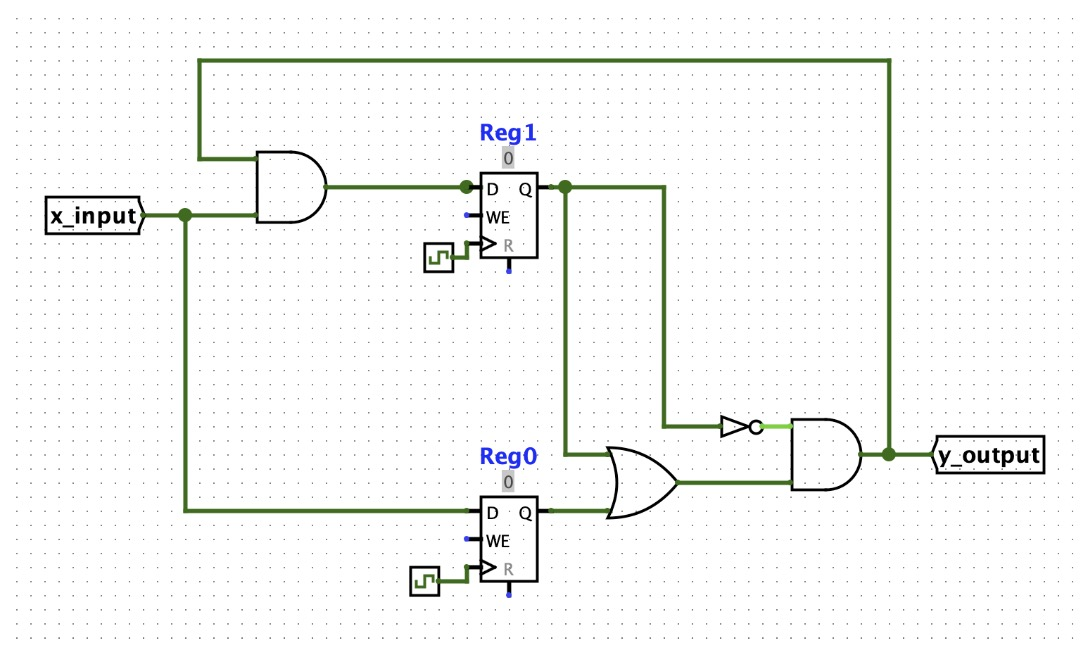
\includegraphics[width=\textwidth]{sds/su20FinalQ4_circuit}

\question
For this question, assume:
\begin{itemize}
	\item \textbf{AND} gates have a propagation delay of 9ns
	\item \textbf{OR} gates have a propagation delay of 14ns
	\item \textbf{NOT} gates have a propagation delay of 5ns
	\item \textbf{x\_input} switches value 30ns after the rising edge of the clock
	\item \textbf{y\_output} is directly attached to a register
	\item \textbf{Setup} time is 3ns
	\item \textbf{Clk-to-Q} delay is 4ns
\end{itemize}

Given the above circuit diagram, answer the following questions:

\end{blocksection}
\begin{blocksection}

\begin{parts}

\part What is the max hold time in ns?

\begin{solution}[0.5in]
18 ns\newline
Shortest CL between registers: NOT + AND = 5 + 9 = 14ns
Max hold time = Clk-to-Q + Shortest CL = 4 + 14 = 18ns
\end{solution}

\part What is the minimum clock period in ns?

\begin{solution}[0.5in]
42 ns\newline
Critical path = 30ns (for x\_input to change) + 9 (AND) + 3 (Setup) = 42ns
\end{solution}

\part Regardless of your previous answers, assume the clock period is 50ns, the first rising edge of the clock is at 25ns and x\_input is initialized to 0 at 0ns. At what time in ns will y\_output become 1?

\begin{solution}[0.5in]
102 ns\newline
25 (First rising edge) + 50 (clock period) + 4 (Clk-to-Q) + 14 (OR) + 9 (AND) = 102ns
\end{solution}

\part How long will y\_output remain equal to 1 before switching to 0?

\begin{solution}[0.5in]
50ns\newline
If y\_output changes to 1 at 102, the next rising edge is at 125.  From there, it takes Clk-Q (4) +OR (14) + AND (9) = 27 ns to update y\_output to 0 again, so at 125 + 27 = 152 ns, 152 - 102 = 50ns
\end{solution}

\end{parts}

\end{blocksection}